\documentclass{standalone}
\usepackage{tikz}
\begin{document}
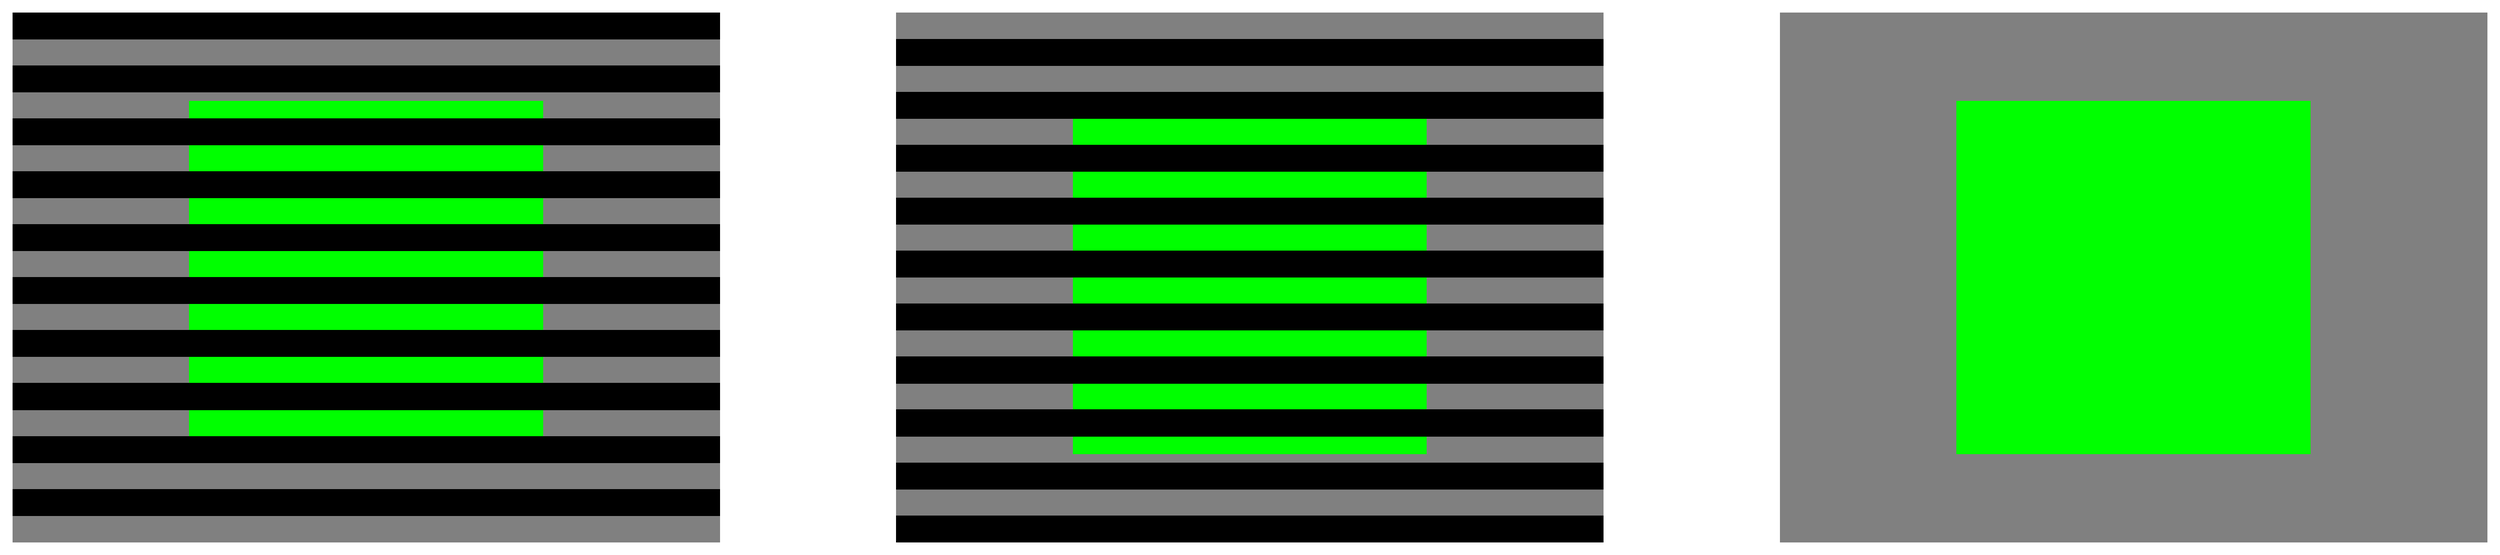
\begin{tikzpicture}[scale=5]

\def\wid{4.0}
\def\hei{3.0}
\def\spheresize{1.0}
\def\clrback{gray}
\def\clrsphere{green}
\def\clrlines{black}
\def\numlines{20}
\def\lastline{19}

\newcommand*{\scene}[1]{
	\draw [\clrback,fill] (#1,0) rectangle (#1+\wid,\hei);

	% circle confuses the image because of its seemingly higher-than-pixelrow resolution in curves :(
	%\draw [\clrsphere,fill] (#1+\wid/2,\hei/2) circle [radius=\spheresize];
	\draw [\clrsphere,fill] (#1+\wid/2-\spheresize,\hei/2-\spheresize) rectangle (#1+\wid/2+\spheresize,\hei/2+\spheresize);
}

\newcommand*{\scenefull}[2]{
	\scene{#1}
	\foreach \y in {#2,...,\lastline} { % ,...,\numlines} {
		\draw [\clrlines,fill] (#1,\y*\hei/\numlines) rectangle (#1+\wid,{(\y+1)*\hei/\numlines});
	}
}

\scenefull{0}{1,3}
\scenefull{5}{0,2}
\scene{10}

\end{tikzpicture}
\end{document}
